Este manual esta diseñado para ayudar al usuario a utilizar el sistema de manera efectiva y realizar consultasbooleanas en tus documentos. El sistema permite buscar documentos que contienen palabras clave especificas
utilizando operadores logicos como AND, OR y NOT.
\subsection{Interfaz}
En la parte de la izquierda, podemos ver una entrada de texto, para ingresar la consulta, a su vez, un
boton para realizar las operaciones de la consulta y un boton de ”ayuda”para ver como se debe ingresar
la consulta. Mas abajo, podemos ver un cuadro de texto en donde se ven todos los documentos que se
encuentran los documentos.
En la parte de la derecha, habra un espacio de texto para ver el contenido de los documentos de texto que
se encuentra en el archivo.
\begin{figure}[ht]
  \centering
  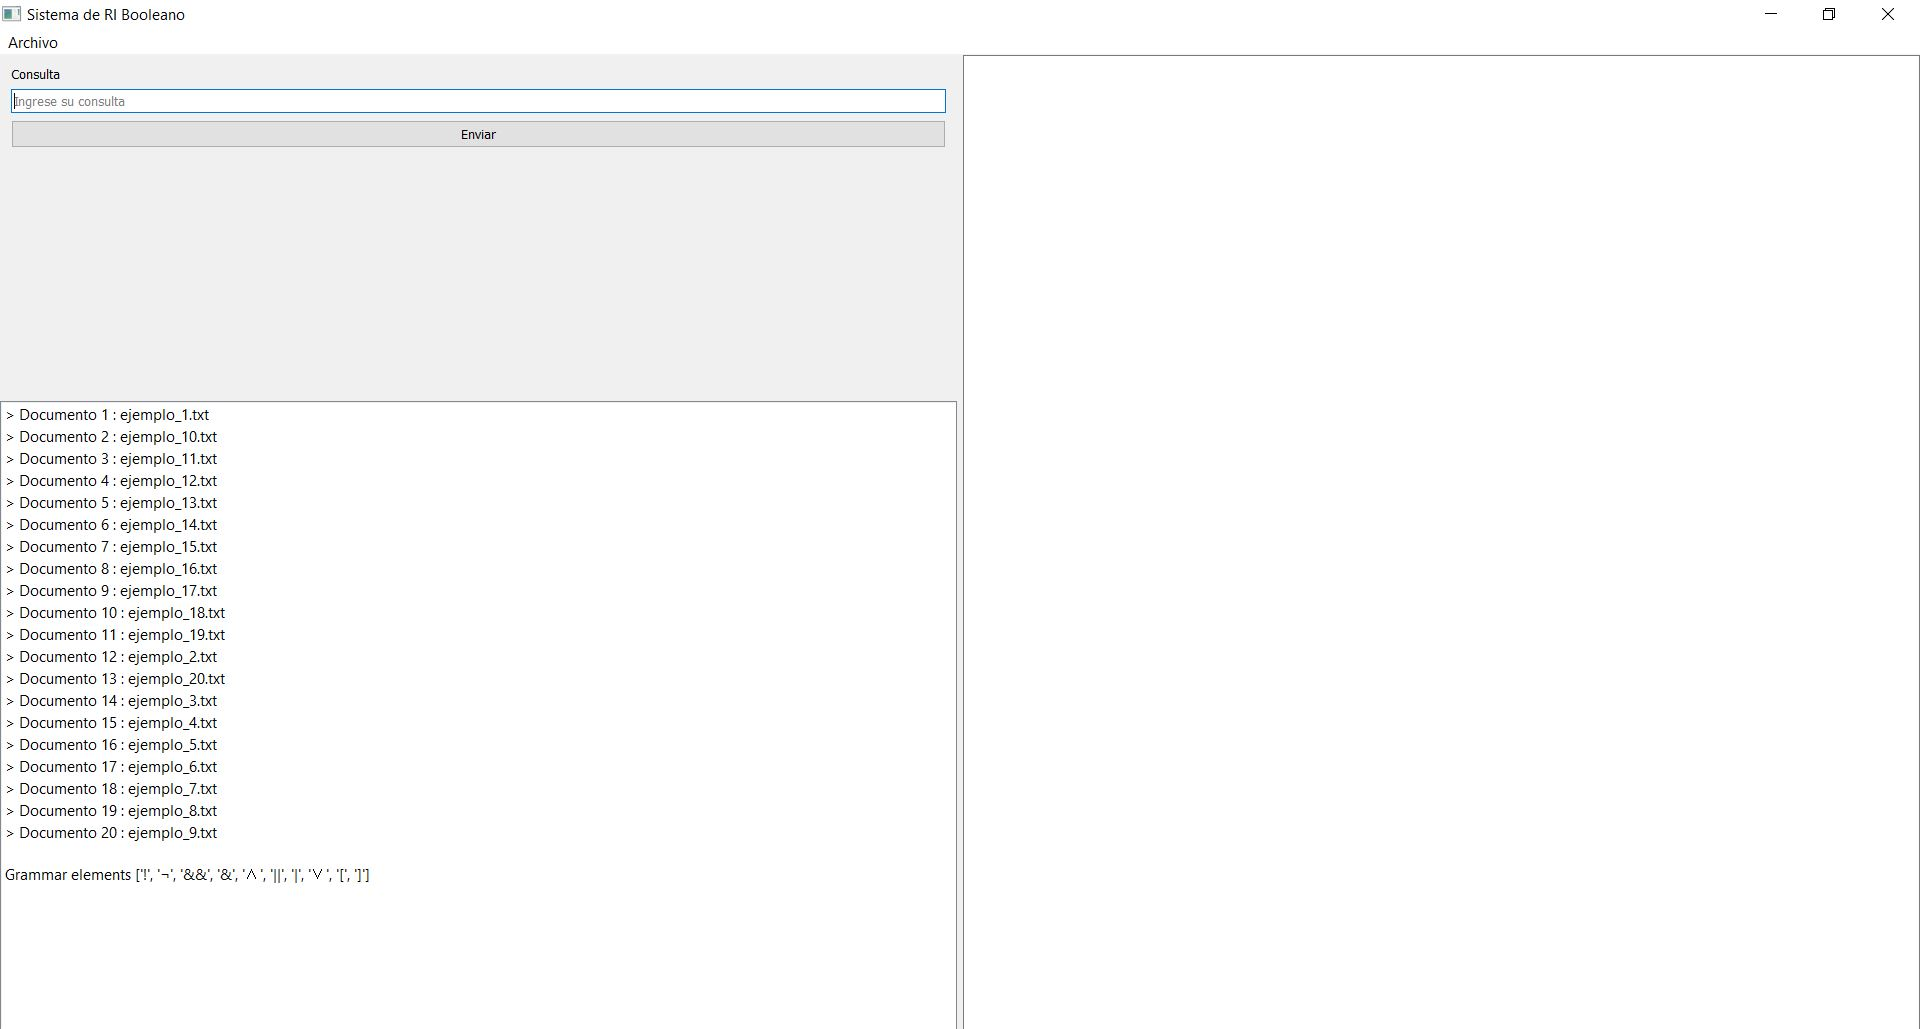
\includegraphics[width=0.8\textwidth]{src/img/ejecucion/1.jpg}
  \caption{Interfaz del sistema}
\end{figure}
\subsection*{Boton de ayuda}
Con este boton, el programa nos lanzara una ventana para que nos aconseje como se debe de ingresar la
consulta.
\begin{figure}[ht]
  \centering
  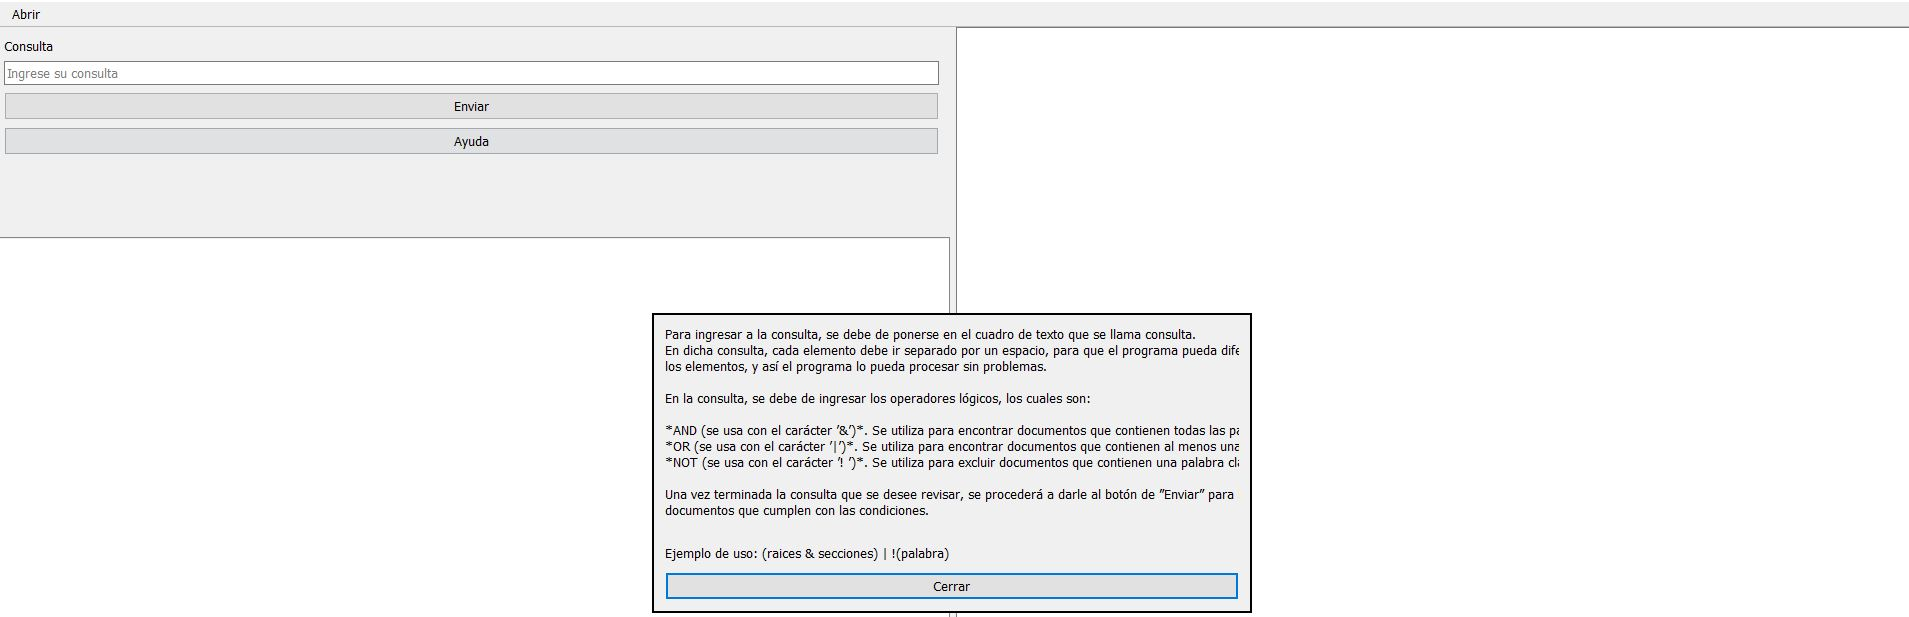
\includegraphics[width=0.8\textwidth]{src/img/ejecucion/2.jpg}
  \caption{Interfaz del sistema}
\end{figure}
\subsection{Visualizar documentos}
Para poder el contenido de los documentos, simplemente se debe de dar clic a cualquiera de los documentos
desplegados en la Interfaz, y en la parte derecha de la interfaz se desplegara el contenido de dicho
documentos.
\begin{figure}[ht]
  \centering
  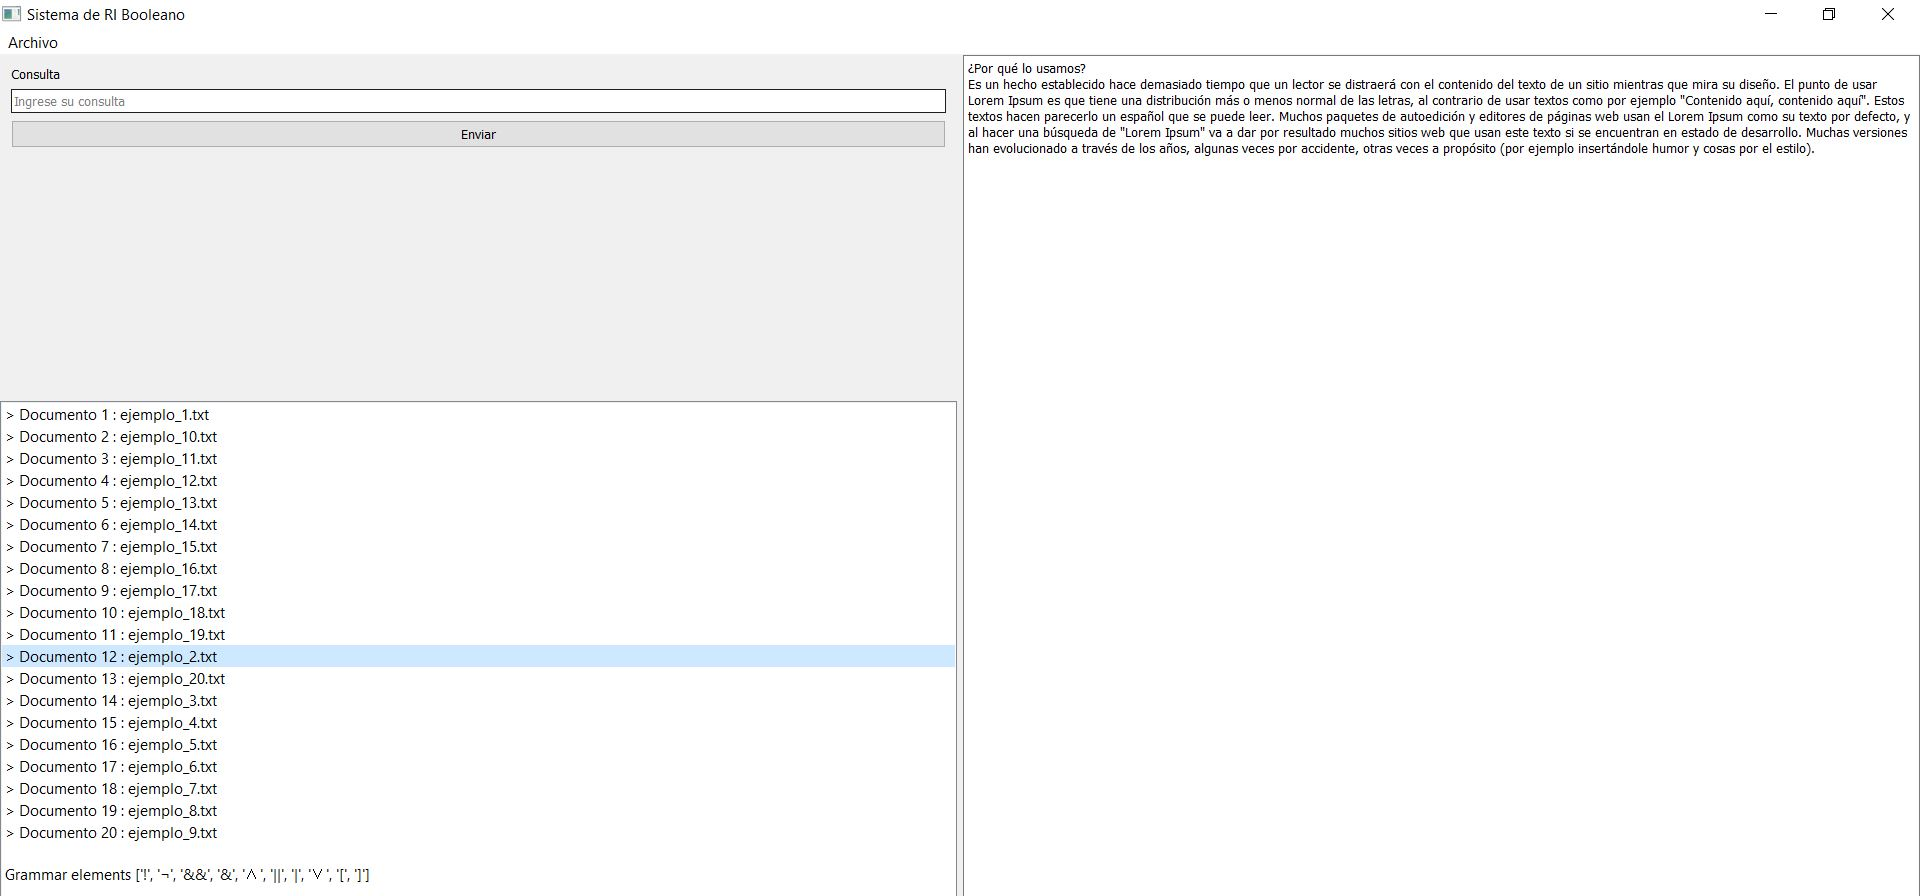
\includegraphics[width=0.8\textwidth]{src/img/ejecucion/3.jpg}
  \caption{Interfaz del sistema}
\end{figure}
\subsection{Realizar Consultas}
Cada elemento de la consulta, debe ir separados por un espacio, para que el programa pueda diferenciar
cada uno de los elementos de la consulta, y asi el programa lo pueda procesar sin problemas. En la consulta,
se debe de usar los operadores logicos, los cuales son:
\begin{itemize}
  \item De tipo AND (representado en el programa como ’\&'). Se utiliza para encontrar documentos que
        contienen todas las palabras clave.
  \item De tipo OR (representado en el programa como ’$\|$’): Se utiliza para encontrar documentos que contienen
        al menos una de las palabras clave.
  \item De tipo NOT (representado en el programa como ’\!’): Se utiliza para excluir documentos que contienen
        una palabra clave especifica.
\end{itemize}
Una vez terminada la consulta que se desee revisar, se procedera a a darle al boton de ”Enviar”para
proceder a hacer el metodo que permitira evaluar los documentos que cumplen con las condiciones de la
consulta. Dicha evaluacion, se hara mediante la notacion Post-Fija.
La notacion Post-Fija es importante debido a que permite evaluar expresiones booleanas de manera
eficiente utilizando una pila (stack) en lugar de requerir una analisis de precedencia de operadores. Esto
simplifica significativamente la logica de procesamiento de consultas booleanas y reduce la complejidad
del codigo. Esto hace que la notacion no contenga ambig¨uedades debido a la secuencia de operadores y
operandos dicta el orden de evaluacion. A su vez, la implementacion se puede implementar de manera
sencilla mediante una pila, lo que simplifica la logica del programa. Por lo que cada operando se empuja
a la pila, y cuando se encuentra un operador, se sacan los operandos necesarios de la pila para realizar
la operacion. Esto hace que el codigo sea mas claro y menos propenso a errores. Algunos ejemplos para
realizar la consulta son:
\subsubsection{consulta 1}
( ( perro $\|$ gato ) \& ( ( ! ( delfin $\|$ oso ) ) \&  lobo ) ) \newline
Query Expresion List: ['[', 'perr', '|', 'gat', ']', '\&', ' [', '[', '!', '[', 'delfin', '|', 'oso', ']', ']', '\&', 'lob', ']']
Stem Elements['perr', 'gat', 'delfin', 'oso', 'lob']

Procesamiento 1
\newline Stack Temp: ['[']
\newline Expresion Postfijo: []


Procesamiento 2
\newline Stack Temp: ['[']
\newline Expresion Postfijo: ['perr']


Procesamiento 3
\newline Stack Temp: ['[', '$\|$']
\newline Expresion Postfijo: ['perr']


Procesamiento 4
\newline Stack Temp: ['[', '$\|$']
\newline Expresion Postfijo: ['perr', 'gat']


Procesamiento 5
\newline Stack Temp: []
\newline Expresion Postfijo: ['perr', 'gat', '$\|$']


Procesamiento 6
\newline Stack Temp: ['\&']
\newline Expresion Postfijo: ['perr', 'gat', '$\|$']


Procesamiento 7
\newline Stack Temp: ['\&', '[']
\newline Expresion Postfijo: ['perr', 'gat', '$\|$']


Procesamiento 8
\newline Stack Temp: ['\&', '[', '[']
\newline Expresion Postfijo: ['perr', 'gat', '$\|$']


Procesamiento 9
\newline Stack Temp: ['\&', '[', '[', '\!']
\newline Expresion Postfijo: ['perr', 'gat', '$\|$']


Procesamiento 10
\newline Stack Temp: ['\&', '[', '[', '\!', '[']
\newline Expresion Postfijo: ['perr', 'gat', '$\|$']


Procesamiento 11
\newline Stack Temp: ['\&', '[', '[', '\!', '[']
\newline Expresion Postfijo: ['perr', 'gat', '$\|$', 'delfin']


Procesamiento 12
\newline Stack Temp: ['\&', '[', '[', '\!', '[', '$\|$']
\newline Expresion Postfijo: ['perr', 'gat', '$\|$',  'delfin']


Procesamiento 13
\newline Stack Temp: ['\&', '[', '[', '\!', '[', '$\|$']
\newline Expresion Postfijo: ['perr', 'gat', '$\|$', 'delfin', 'oso']


Procesamiento 14
\newline Stack Temp: ['\&', '[', '[', '\!']
\newline Expresion Postfijo: ['perr', 'gat', '$\|$', 'delfin', 'oso', '$\|$']


Procesamiento 15
\newline Stack Temp: ['\&', '[']
\newline Expresion Postfijo: ['perr', 'gat', '$\|$', 'delfin', 'oso', '$\|$', '\!']


Procesamiento 16
\newline Stack Temp: ['\&', '[', '\&']
\newline Expresion Postfijo: ['perr', 'gat', '$\|$', 'delfin', 'oso', '$\|$', '\!']


Procesamiento 17
\newline Stack Temp: ['\&', '[', '\&']
\newline Expresion Postfijo: ['perr', 'gat', '$\|$', 'delfin', 'oso', '$\|$', '\!', 'lob']


Procesamiento 18
\newline Stack Temp: []
\newline Expresion Postfijo: ['perr', 'gat', '$\|$', 'delfin', 'oso', '$\|$', '\!', 'lob', '\&', '\&']

Expresion Postfijo Final: ['perr', 'gat', '$\|$', 'delfin', 'oso', '$\|$', '\!', 'lob', '\&', '\&']

Procesamiento de la consulta:

$'perr': ['ejemplo_3.txt', 'ejemplo_4.txt', 'ejemplo_5.txt']$

'gat': ['$ejemplo_2.txt$', '$ejemplo_3.txt$', '$ejemplo_4.txt$']

Operador $\|\|$ (or) seleccionado

$['ejemplo_3.txt', 'ejemplo_4.txt', 'ejemplo_5.txt'] \lor ['ejemplo_2.txt', 'ejemplo_3.txt', 'ejemplo_4.txt']$

$['ejemplo_2.txt', 'ejemplo_3.txt', 'ejemplo_4.txt', 'ejemplo_5.txt']$

'delfin': ['$ejemplo_1.txt$', '$ejemplo_2.txt$', '$ejemplo_4.txt$']

'oso': ['$ejemplo_1.txt$', '$ejemplo_4.txt$', '$ejemplo_5.txt$']

Operador $\|\|$ (or) seleccionado

$['ejemplo_1.txt', 'ejemplo_2.txt', 'ejemplo_4.txt'] \lor ['ejemplo_1.txt', 'ejemplo_4.txt', 'ejemplo_5.txt']$

$['ejemplo_1.txt', 'ejemplo_2.txt', 'ejemplo_4.txt', 'ejemplo_5.txt']$

Operador ! (not) seleccionado

$\neg['ejemplo_1.txt', 'ejemplo_2.txt', 'ejemplo_4.txt', 'ejemplo_5.txt']$

$['ejemplo_3.txt']$

'lob': ['$ejemplo_1.txt$', '$ejemplo_2.txt$', '$ejemplo_3.txt$', '$ejemplo_4.txt$']

Operador \&\& (and) seleccionado

$['ejemplo_3.txt'] \land ['ejemplo_1.txt', 'ejemplo_2.txt', 'ejemplo_3.txt', 'ejemplo_4.txt']$

$['ejemplo_3.txt']$

Operador \&\& (and) seleccionado

$['ejemplo_2.txt', 'ejemplo_3.txt', 'ejemplo_4.txt', 'ejemplo_5.txt'] \land ['ejemplo_3.txt']$

$['ejemplo_3.txt']$

Documentos que satisfacen la consulta:

> Documento 3 : $ejemplo_3.txt$

\begin{figure}[ht]
  \centering
  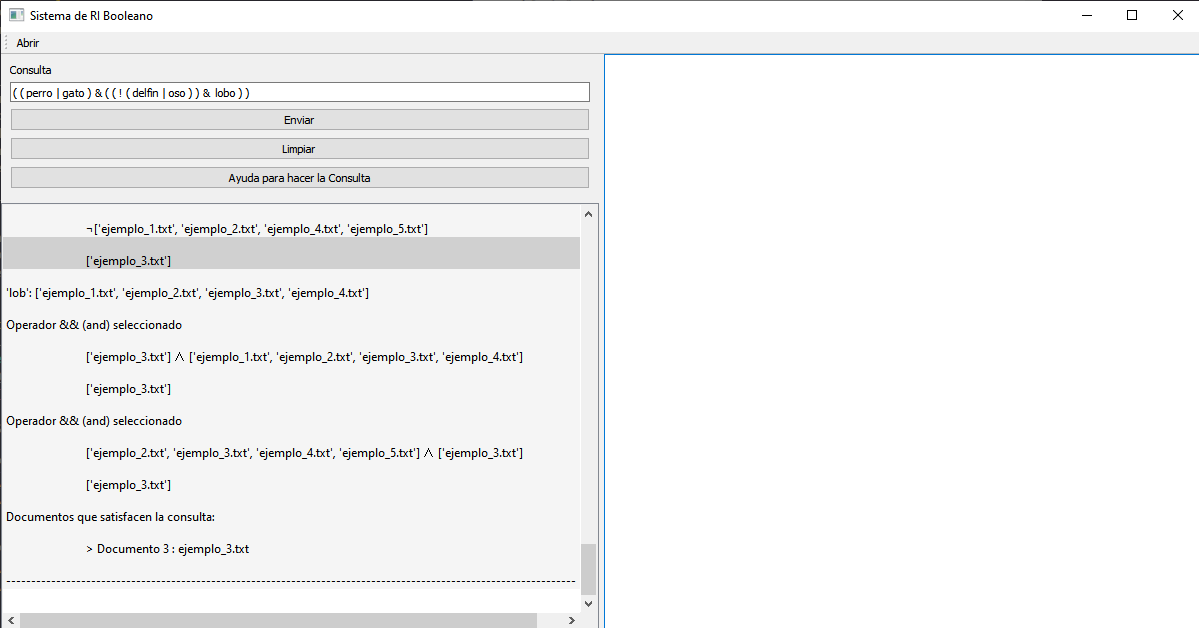
\includegraphics[width=0.8\textwidth]{src/img/ejecucion/4.png}
  \caption{Interfaz del sistema}
\end{figure}
\newpage
\subsubsection{consulta 2}
( ( perro $\|$ gato ) \& ( ( ! ( delfin ) $\|$ oso )  \&  lobo ) )
\begin{figure}[ht]
  \centering
  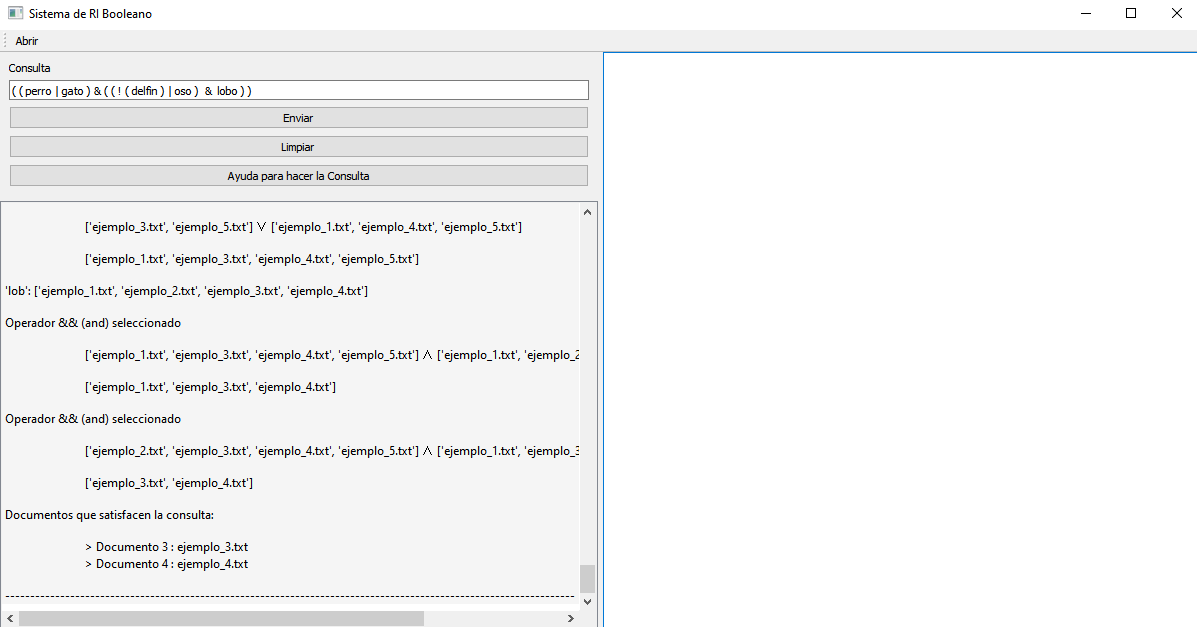
\includegraphics[width=0.8\textwidth]{src/img/ejecucion/5.png}
  \caption{Interfaz del sistema}
\end{figure}

